
\section{Versuchsaufbau und Durchführung}

\noindent
Für diesen Versuch wird ein Ultraschallechoskop mit angeschlossener Ultaschallsonde, für das Echo-Impuls-Verfahren, genutzt.\\
Das Gerät ist dabei an einen Computer angeschlossen mit dem sich die Messwerte auswerten lassen können.
Dabei lassen sich die Sende, sowie die Empfangsleistung und die jeweiligen Laufzeiten im Impuls-Betrieb, vom Programm EchoView auslesen.\\\\

\noindent
Zuerst soll ein Plexiglasblock mit Lufteinschlüssen unterschiedlicher Größe bei unterschiedlichen Tiefen untersucht werden.\\
Der Block und dabei auch der Ort der Einschlüsse wird zuerst mit einem Messschieber vermessen um Referenzwerte zu erhalten.\\
Nun wird als Kontaktmittel bidestiliertes auf den Block aufgetragen. 
Anschließend wird dann die Ultraschallsonde über den Block gefahren und für jeden Lufteinschluss vom Computer die Laufzeit des Impulses und die gemessene reflektierte Intensität gemessen.\\
Dieselbe Messung wird dann für die andere Seite des Blocks wiederholt.

\begin{figure}
    \centering
    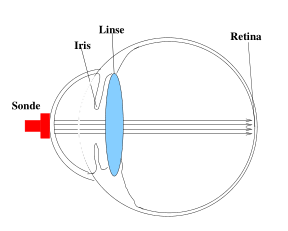
\includegraphics[width=0.65\textwidth]{latex/images/auge.PNG}
    \caption{Schematische Darstellung des Augenmodells, welche zu untersuchen istS\protect \cite{US1}.}
    \label{img:auge}
\end{figure}

\noindent
Als nächste Messreihe soll ein Modell eines Auges untersucht werden. Dieses ist in Abbildung \ref{img:auge} dargestellt.\\
Auf das Linse des Modells wird wieder das Kontaktmittel aufgetragen. Mit der Sonde kann dann das Innere des Auges untersucht werden.\\
Dies geschieht über die Interpretation der unterschiedlichen reflektierten Impulse, die im Messprogramm abgebildet werden.

